\documentclass[11pt, twocolumn]{article}
\usepackage{lingmacros}
\usepackage{tree-dvips}
\usepackage{graphicx}
\usepackage{amsmath}
\usepackage{amssymb}
\usepackage{tikz}
\usepackage{color}
\usepackage{comment}

\begin{document}

\title{Performance Evaluation of Automatic Differentiation Algorithms for Hessian Computation}
\maketitle

\section*{Introduction}
The second order derivative of a scalar function, i.e, the Hessian matrix, plays 
an important role in many applications. 
Several Automatic Differentiation (AD)-based Hessian evaluation algorithms have been proposed and implemented in the literature. While the high-level differences between the algorithms is generally understood, the detailed behavior of the algorithms and their performance characterization with respect to the structure and complexity of the computer code  representing the function to be differentiated has not been systematically studied and understood. In this work, we design a synthetic function that allows us to change the structural properties of the function by tuning parameters, and we use the designed function to study the performance of four different Hessian computation algorithms and the sensitivity of the performance to variations in those structural properties.

\section*{Algorithms}

We study three different approaches for Hessian evaluation. The first approach in turn has two variants, and so in total we consider four algorithms. In all four algorithms, 
the sparsity available in the final Hessian is exploited; that is, computing with and storing zero entries is avoided.  

{\bf (i) Compression-based methods:}
The first two methods se study are based on the {\em forward-over-reverse mode}, or {\em Second-Order-Adjoint-Mode (SOAM)}, of Automatic Differentiation~\cite{griewank2008evaluating, naumann2012art}. Each run of a forward-over-reverse mode gives a Hessian-vector product $Hv$. Thus a trivial approach to get the entire Hessian matrix is to run the forward-over-reverse mode $n$ times, where $n$ is the number of columns in the Hessian and each run evaluates the $i$-th column of the Hessian, $He_i$. This approach is clearly not efficient  when the Hessian matrix is sparse.  Therefore a compression-based method is used instead \cite{gebremedhin2009efficient}. 

The idea behind compression-based approach is to determine an $n$ by $p$ seed matrix $S$
that encodes the set columns of the Hessian that can be ``compressed" together and evaluated via one Hessian-vector product. The seed matrix is typically obtained by
coloring the graph associated with the sparsity pattern of the Hessian. 
The number of columns $p$ in the seed matrix is exactly the number of colors needed. 
In this manner, only $p$ Hessian-vector products, instead of $n \gg p$ Hessan-vector products, is needed to obtain a compressed version of the Hessian. The desired Hessian is then obtained via a suitable recovery step.  

Depending on how the recovery step is to be performed, two different kinds of coloring are needed in the determination of the seed matrix. If the recovery is direct (no further arithmetic is involved in obtaining entries of the original Hessian),  {\em star} coloring is the needed coloring;
and if the recovery is indirect (entries of the original Hessian are obtained via substitutions), {\em acyclic} coloring is what is needed. In what follows, we refer to these two approaches  as {\tt Direct} and {\tt Indirect} respectively. We use the implementations in {\tt ADOL-C} \cite{walther2009getting} and {\tt ColPack} \cite{gebremedhin2013colpack}, in which {\tt ADOL-C} is responsible for the routines corresponding to computing the sparsity pattern and evaluating the compressed Hessian, and {\tt COlPack} is responsible for the routines  corresponding to coloring the adjacency graph and recovery the Hessian from the compressed representation.

{\bf (ii) Taylor coefficient based method. } 
The third Hessian evaluation method  we study  corresponds to evaluating the Hessian by propagating a family of second order Taylor coefficients~\cite{griewank2000evaluating}. 
By assigning pre-calculated initial values for each Taylor series, each entry in the Hessian matrix  can be determined by a linear combination of the final Taylor coefficients. Each initial value is called a {\em direction}.
The complexity of evaluating the Hessian using this method is proportional to a combination of $n^2$ and the complexity of the objective function. The complexity can be made proportional to $nnz$ and the complexity of the objective function, where $nnz$ is the number of non-zeros in the final Hessian matrix, by only evaluating those non-zero entries.
%The complexity of this method is $O(n^2)$. And if we know the sparsity pattern of the final Hessian matrix, the complexity can be reduced to $O(nnz)$ where $nnz$ is the number of non-zeros in the final Hessian matrix by only evaluating those non-zero entries.
We use the implementation in {\tt Rapsodia}~\cite{charpentier2009fast} and provide a patch which allows {\tt Rapsodia} to only evaluate the non-zero entries in the Hessian matrix with pre-determined sparsity pattern information. For the latter information, we use the sparsity pattern computed by {\tt ADOL-C}. The design philosophy of {\tt Rapsodia} is to use flat code to evaluate the Taylor coefficients for all directions. Given the number of directions, {\tt Rapsodia} explicitly generates this flat code. As we will show, when the number of directions is large, the generated code is very large and compilation takes huge amounts of time (several hours even for a moderate size problem), making the method infeasible. 

{\bf (iii) Live variable based method. }
The last method we study is second order reverse mode based on the live variable approach \cite{wang2016capitalizing}. The key idea in the algorithm is to extend a useful invariant in reverse mode AD into the second order. In particular, the key insight is that, at each point, the intermediate state of the reverse mode algorithm is the derivative of an equivalent function with respect to the live variable set at that point. The equivalent function is defined by the single assignment code processed in earlier steps. The complexity of this method is proportional to the size of live variable sets and the complexity of the objective function. We implement this algorithm in a tool we called {\tt ReverseAD} and uses this implementation in the comparison.

\section*{Design of test cases}

For our purposes, we needed to generate test cases designed to enable in-depth
empirical analysis of {\em programming} and {\em structural factors} that 
determine the performance of the  different Hessian algorithms we consider. 
To construct such test cases, we wrote a code that works as follows. 
Let the number of rows in the target Hessian matrix be $n$, and
let the average number of nonzeros per row, $\bar{\rho}$, be fixed.
In a loop over the $n$ rows, for each row $i$, 
we pick $\frac{\bar{\rho}}{2}$ column indices at random to insert nonzero values into the Hessian.    
We do this by using a deterministic random number generator to identify a column index $j$ and {\em the basic operation} 
$\tt 1.0+x[i]*x[j]$ to create the nonzero entry in the location $H(i,j)$. 
Further, a statement in the loop consists of the sum of $k$ basic operations added to the dependent variable $y$. We also permit a statement to be repeated $s$ times in a loop. Thus the total number of basic operations per loop is the product of the number of statements per loop $s$ and the number of basic operations per statement $k$. 
Varying $s$ and $k$ gives us the flexibility to implement the same function in different ways.

Within this setting, we can control the number of rows in the Hessian matrix, the density/sparsity of the Hessian, and the complexity of the function evaluation. 
%Because we build the objective function in a ``separable'' fashion, in the complexity of 
%\textsc{Livarh} given by Expression~\eqref{eq-ub1}, $d_i$ is constant, which means the complexity of \textsc{Livarh} is proportional to just $l$, the complexity of the function 
%evaluation in this case.
We include pseudocode for the random Hessian generator we described in 
Figure~\ref{fig:RandomHessianGenerator} in the Appendix.
%the Appendix~\ref{sec-random-code}.)   

\begin{comment}
We construct testcases specially designed to enable in-depth empirical analysis of {\em structural factors} that determine the performance of the  different Hessian algorithms. 
To construct the testcases, we wrote a simple code that works as follows. 
Let the number of rows in the target Hessian matrix be $n$, and let the average number of nonzeros per row, $\bar{\rho}$, be fixed.
In a loop over the $n$ rows, we randomly pick $\frac{\bar{\rho}}{2}$ column indices $j$ and create a nonzero entry in the location $H(i,j)$. During the creation, we duplicate $s$ copies of $x[i]$ to maintain that the size of live variable sets during the function evaluation to be $s$ for the most of the time. And we also let $x[i]$ to pass through $k$ identity functions to make sure the test function covers a variety of kinds of operators and elementary functions. And this also provides a way to allow us control the complexity of the function evaluation. Each identity function is randomly chosen among six pre-determined forms. 

%In a loop over the $n$ rows, for each row $i$, we pick $\frac{\bar{\rho}}{2}$ column indices at random to insert nonzero values into the Hessian. We do this by randomly pick a column index $j$ and use {\em the basic operation} $t_{ij} = \tt 1.0+x[i]*x[j]$ to create the nonzero entry in the location $H(i,j)$. 
%Then, we let $t_{ij}$ to pass through $k$ identify functions. Each identity function is randomly choose among six pre-determined forms. This is to make sure that the test function covers a variety of kinds of operators and elementary functions.
All random numbers are generated by a deterministic random number generator. So we can repeat the exact same function evaluation by giving the same initial random seed.

So with this setting, we can control the number of rows in the Hessian matrix $n$, the density/sparsity of the Hessian $\rho$, and the complexity of the function evaluation $k$, and the size of live variable sets during the function evaluation $s$.
%Because we build the objective function in a ``separable'' fashion, in the complexity of \textsc{Livarh} given by Expression~\eqref{eq-ub1}, $d_i$ is constant, which means the complexity of \textsc{Livarh} is proportional to just $l$, the complexity of the function evaluation in this case.
\end{comment}

\section*{Results}

\paragraph{(a) General Runtime} We first use some small tests to get a general sense of the performance of the algorithms. We set $\rho = 6$, $k = 30$ and $s = 30$. 
Table~\ref{tab:general} lists the results we obtained when
we run the four algorithms with different values of $n$.  The observation here is that
{\tt Rapsodia} takes much longer time compared with the other three methods, and it also takes hours to compile the ``flat-code'' when there are more than $10,000$ directions. 
So we excludes this method from further tests we report on.
\begin{table*}[htbp]
\begin{center}
\begin{tabular}{ | c | r | r | r | r | r |}
\hline
$n$ & $\#nnz$ in $H$ & {\tt Direct} & {\tt Indirect} & {\tt Rapsodia} & {\tt ReverseAD} \\
\hline
$2,000$ & 7,990 & 2.332 & 1.996 & 11.703 & 0.795 \\
$3,000$ & 11,989 & 3.671 & 3.258 & 26.808 & 1.207\\
\hline 
\end{tabular}
\caption{General Runtime for {\tt Direct}, {\tt Indirect}, {\tt Rapsodia} and {\tt ReverseAD}.}
\label{tab:general}
\end{center}
\end{table*}

\paragraph{(b) Function Complexity} 
Our goal here is to see how the performance changes as the function complexity is varied.
We set $n = 20,000$, $\rho = 6$, $s = 30$, and vary $k$ from $20$ to $60$. 
We found that the runtime of {\tt Direct} and {\tt Indirect} increases super-linearly with increase in the function complexity. Further, we found that that more than $90\%$ (or $99\%$ in the last two tests) of the time is spent in the sparsity pattern detection procedure. It is likely that our synthetic function is among the ``worst-case" instances for the current sparsity pattern detection procedure implemented in ADOL-C.  Finally, we see that the runtime of {\tt ReverseAD} is within the same order of the function complexity.
\begin{table*}[htbp]
\begin{center}
\begin{tabular}{ | c | r | r | r | r | r |}
\hline
 & $k=$ 20 & 30 & 40 & 50 & 60 \\
\hline
{\tt Direct} & 9.325 & 25.268 &181.435 &1765.766 & 14114.265\\
{\tt Indirect} & 7.138 & 22.007 & 177.539 & 1760.754 & 14124.760\\
{\tt ReverseAD}  & 6.367 & 8.220 & 9.824 & 11.763 & 13.242\\
\hline 
\end{tabular}
\caption{Runtime for {\tt Direct}, {\tt Indirect} and {\tt ReverseAD} with different function complexity.}
\label{tab:complexity}
\end{center}
\end{table*}

\paragraph{(c) Size of Live Variables} 
Here we want to see how the performance changes as we vary the size of the live variable set.
We fix $n = 20,000$, $\rho = 6$, $k = 30$ and changes $s$ from $20$ to $60$. The result suggests that performance of {\tt ReverseAD} is much more sensitive to the size of live variable set than the other two algorithms. This is in accordance with our expectation and the complexity analysis of the algorithm.
\begin{table*}[htbp]
\begin{center}
\begin{tabular}{ | c | r | r | r | r | r |}
\hline
& $s=$ 20 & 30 & 40 & 50 & 60 \\
\hline
{\tt Direct} & 23.653 & 25.138 & 26.484 & 27.666 & 29.208\\
{\tt Indirect} & 21.071 & 22.310 & 23.110 & 23.843 & 25.075\\
{\tt ReverseAD} & 6.137 & 8.087 & 10.207 & 12.507 & 14.421\\
\hline 
\end{tabular}
\caption{Runtime for {\tt Direct}, {\tt Indirect} and {\tt ReverseAD} with different size of live variables.}
\label{tab:live}
\end{center}
\end{table*}

\paragraph{(d) Sparsity/Density} 
Here we fix $s$ to be  $30$, and perform tests on four sets of settings: 
\newline $n=10,000$, $\rho = 12$, $k=60$; 
\newline $n=15,000$, $\rho = 8$, $k=40$; 
\newline $n=20,000$, $\rho=6$, $k=30$; 
\newline $n=30,000$, $\rho=4$, $k=20$. 

We choose those parameters so that the complexity of the function evaluation and the total number of non-zeros in the final Hessian matrix are roughly the same among different settings. 
Table~\ref{tab:sparsity} lists the results we obtained.
We see that the runtime of {\tt Direct} and {\tt Indirect} increases as the density of the Hessian matrix increases. Further, {\tt ReverseAD} takes more time when the density of the Hessian matrix increases, but the growth rate is relatively small.
\begin{table}[htbp]
\begin{center}
\begin{tabular}{ | c | r | r | r |}
\hline
& $k=$ $15,000$ & $20,000$ & $30,000$\\
\hline
{\tt Direct} & 139.841 & 25.745 & 12.833\\
{\tt Indirect} & 134.210 & 22.232 & 9.664 \\
{\tt ReverseAD} & 7.616 & 8.634 & 9.745\\
\hline 
\end{tabular}
\caption{Runtime for {\tt Direct}, {\tt Indirect} and {\tt ReverseAD} with different sparsity/density.}
\label{tab:sparsity}
\end{center}
\end{table}

\section*{Conclusion}
By comparing the performance of the four different Hessian evaluating algorithms, we found that the approach in {\tt Rapsodia} is more suitable when evaluating derivatives for function with a few number of independent variables. We also found that the bottleneck in the compression based methods is mainly the sparsity pattern step. 
The {\tt ReverseAD} approach is more stable and efficient approach in most cases. 

\newpage
\appendix
\subsection{Pseudocode of The Random Hessian Generator}
\label{sec-random-code}

The pseudocode of the random Hessian generator is given in Figure~\ref{fig:RandomHessianGenerator}.

\begin{figure*}
\begin{center}
\begin{tabular*}{\textwidth}{l}
\hline
\textbf{Algorithm:} Random Hessian Generator \\  
\hline
\begin{minipage}{3in}
\begin{verbatim}
// x : array of independent variables
// y : dependent variable
// n : size of the Hessian, y''
// p : half of the average number of nonzeros per row

#define EXP_1 (1.0+x[i]*x[j])  // 1 basic operation to create a nonzero entry
#define EXP_2 EXP_1+EXP_1  // sum of 2 basic operations
#define EXP_4 EXP_2+EXP_2  // sum of 4 basic operations

#define STMT_1_4 y+=EXP_4;  // 1 statement containing 4 basic operations
#define STMT_2_4 STMT_1_4;STMT_1_4;
#define STMT_4_4 STMT_2_4;STMT_2_4;
#define STMT_8_4 STMT_4_4;STMT_4_4;

adouble function random_hess_generator(adouble* x, int n, int p) {
  adouble y=0;
  for(i = 0; i < n; i++) {
    for(l = 0; l < p; l++) {
      j = randomIndex();
      STMT_8_4;  // 8 statements, each containing 4 basic operations
    }
  }
  return y;
}
\end{verbatim}
\end{minipage} \\
\hline
\end{tabular*}
\end{center}
\caption[The Random Hessian Generator]{The Random Hessian Generator. Note that the equivalent mathematical expression is: $y=f(x)=\sum_{i=1}^{i=n} \sum_{l=1}^{l=p} 32 (1.0 + x[i] \times x[j_{il}])$, each $j_{il}$ is randomly chosen from the interval $[1, n]$.}
\label{fig:RandomHessianGenerator}
\end{figure*}

\newpage

\section{The old stuff}
\subsection{Randomized Hessians, Analyzing Program Structures}
\label{sec-perf-rand}

\label{sec-perf-random}

\paragraph{A) Test setting and objectives.}
The objectives of the tests discussed in this section are distinct from
the objectives of the tests presented in Sections~\ref{sec-perf-syn} and \ref{sec-perf-opt}.
Here we construct testcases specially designed to enable in-depth
empirical analysis of {\em programming} and {\em structural factors} that 
determine the performance of the  different Hessian algorithms. 
To construct the testcases, we wrote a simple code that works as follows. 
Let the number of rows in the target Hessian matrix be $n$, and
let the average number of nonzeros per row, $\bar{\rho}$, be fixed.
In a loop over the $n$ rows, for each row $i$, 
we pick $\frac{\bar{\rho}}{2}$ column indices at random to insert nonzero values into the Hessian.    
We do this by using a deterministic random number generator to identify a column index $j$ and {\em the basic operation} 
$\tt 1.0+x[i]*x[j]$ to create the nonzero entry in the location $H(i,j)$. 
Further, a statement in the loop consists of the sum of $k$ basic operations added to the dependent variable $y$. We also permit a statement to be repeated $s$ times in a loop. Thus the total number of basic operations per loop is the product of the number of statements per loop $s$ and the number of basic operations per statement $k$. Varying $s$ and $k$ gives us the flexibility to implement the same function in different ways.

Within this setting, we can control the number of rows in the Hessian matrix, the density/sparsity of the Hessian, and the complexity of the function evaluation. Because we build
the objective function in a ``separable'' fashion, in the complexity of 
\textsc{Livarh} given by Expression~\eqref{eq-ub1}, $d_i$ is constant, which means the complexity of \textsc{Livarh} is proportional to just $l$, the complexity of the function 
evaluation in this case.
(We include pseudocode for the random Hessian generator we described in the Appendix~\ref{sec-random-code}.)   


\paragraph{B) Dependence on number of basic operations per statement.}

As discussed in Section~\ref{sec-preacc-analysis}, the performance of \textsc{Livarhacc} depends on how complex a statement is. We would like to measure this dependence
and see if the other methods' performance also depends on the complexity of a statement. We fix the size of the Hessian as $n=20,000$, the average number of nonzeros per row as $\overline{\rho} = 6$, and the total number of basic operations per loop as $B=128$.
We vary the number of basic operations per statement ($k$) while keeping $B=k s$ fixed, where $s$ is the number of statements per loop. We use a fixed seed in the random number generator,
so we always get the same nonzero structure in the Hessian. 

\begin{figure}[htbp]
\centering
\begin{minipage}[b]{0.48\linewidth}
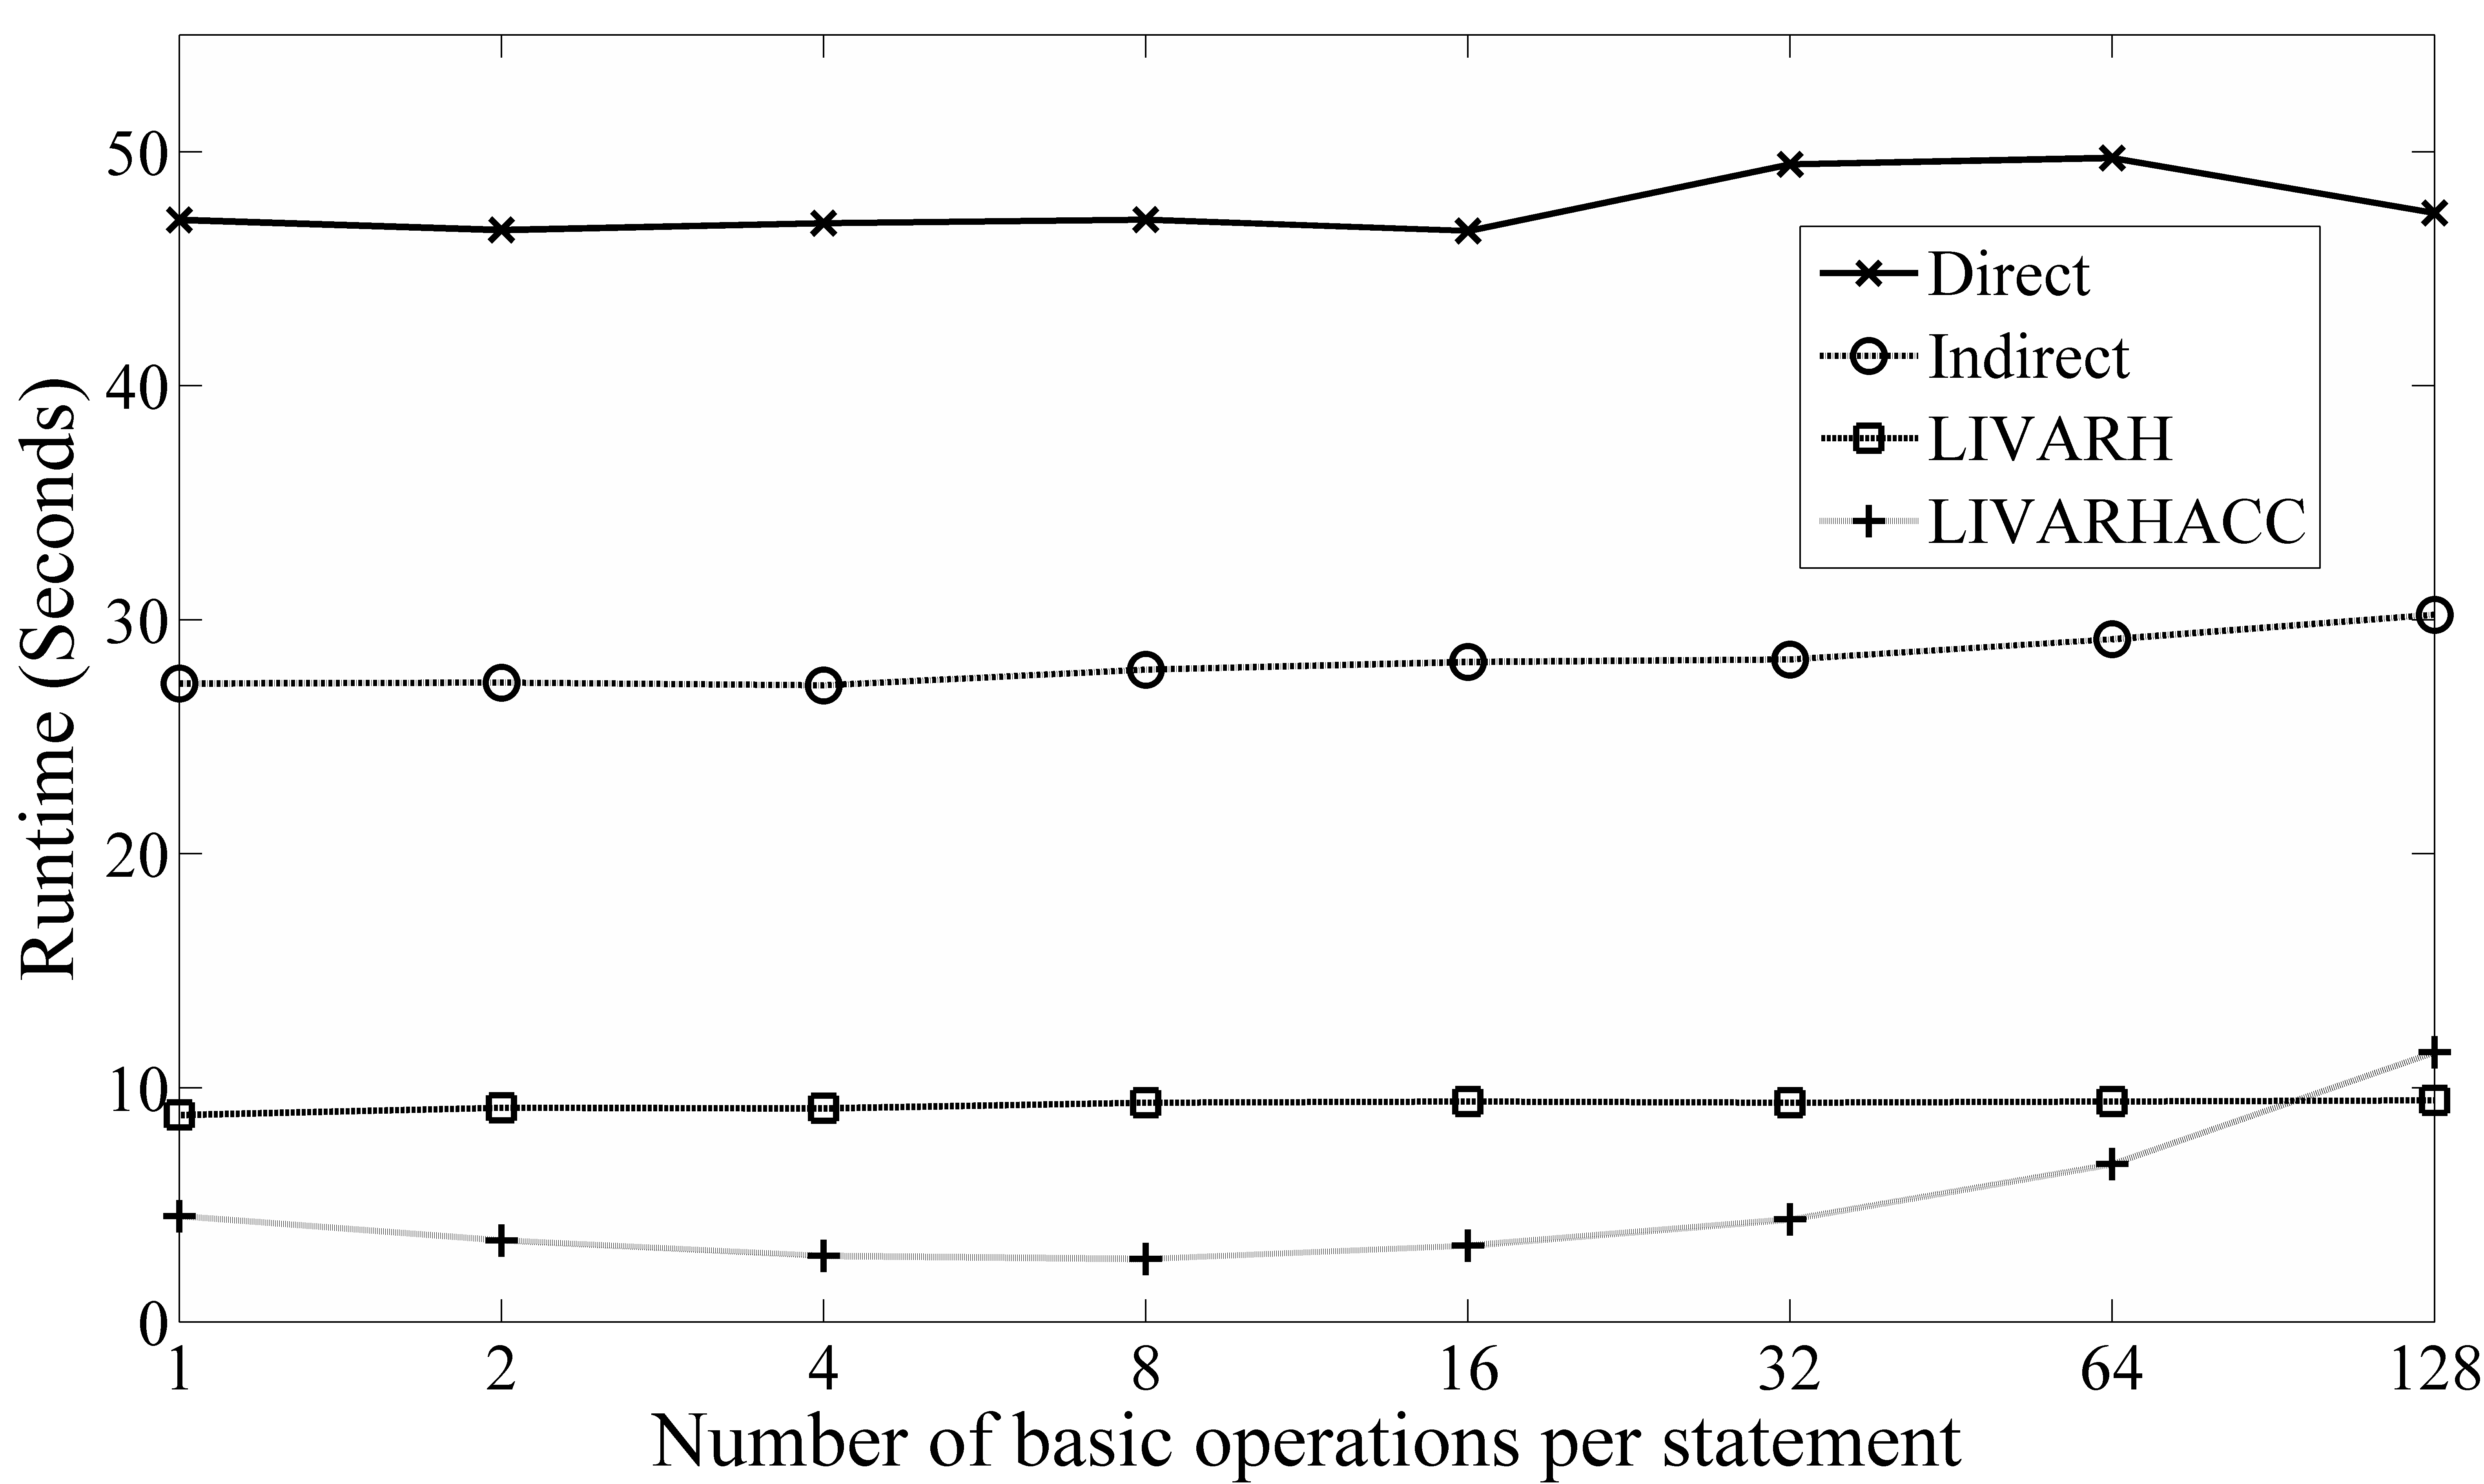
\includegraphics[width=1\textwidth]{figures/HRfig1BW}
\caption[ Runtime Variation under Different Number of Basic Operations per Loop]
{Runtime variation under different number of basic operations per loop.
Fixed parameters: $n=20,000$, $\overline{\rho} = 6$, $B=128$. }
\label{fig:random-fig1}
\end{minipage}
\quad
\begin{minipage}[b]{0.48\linewidth}
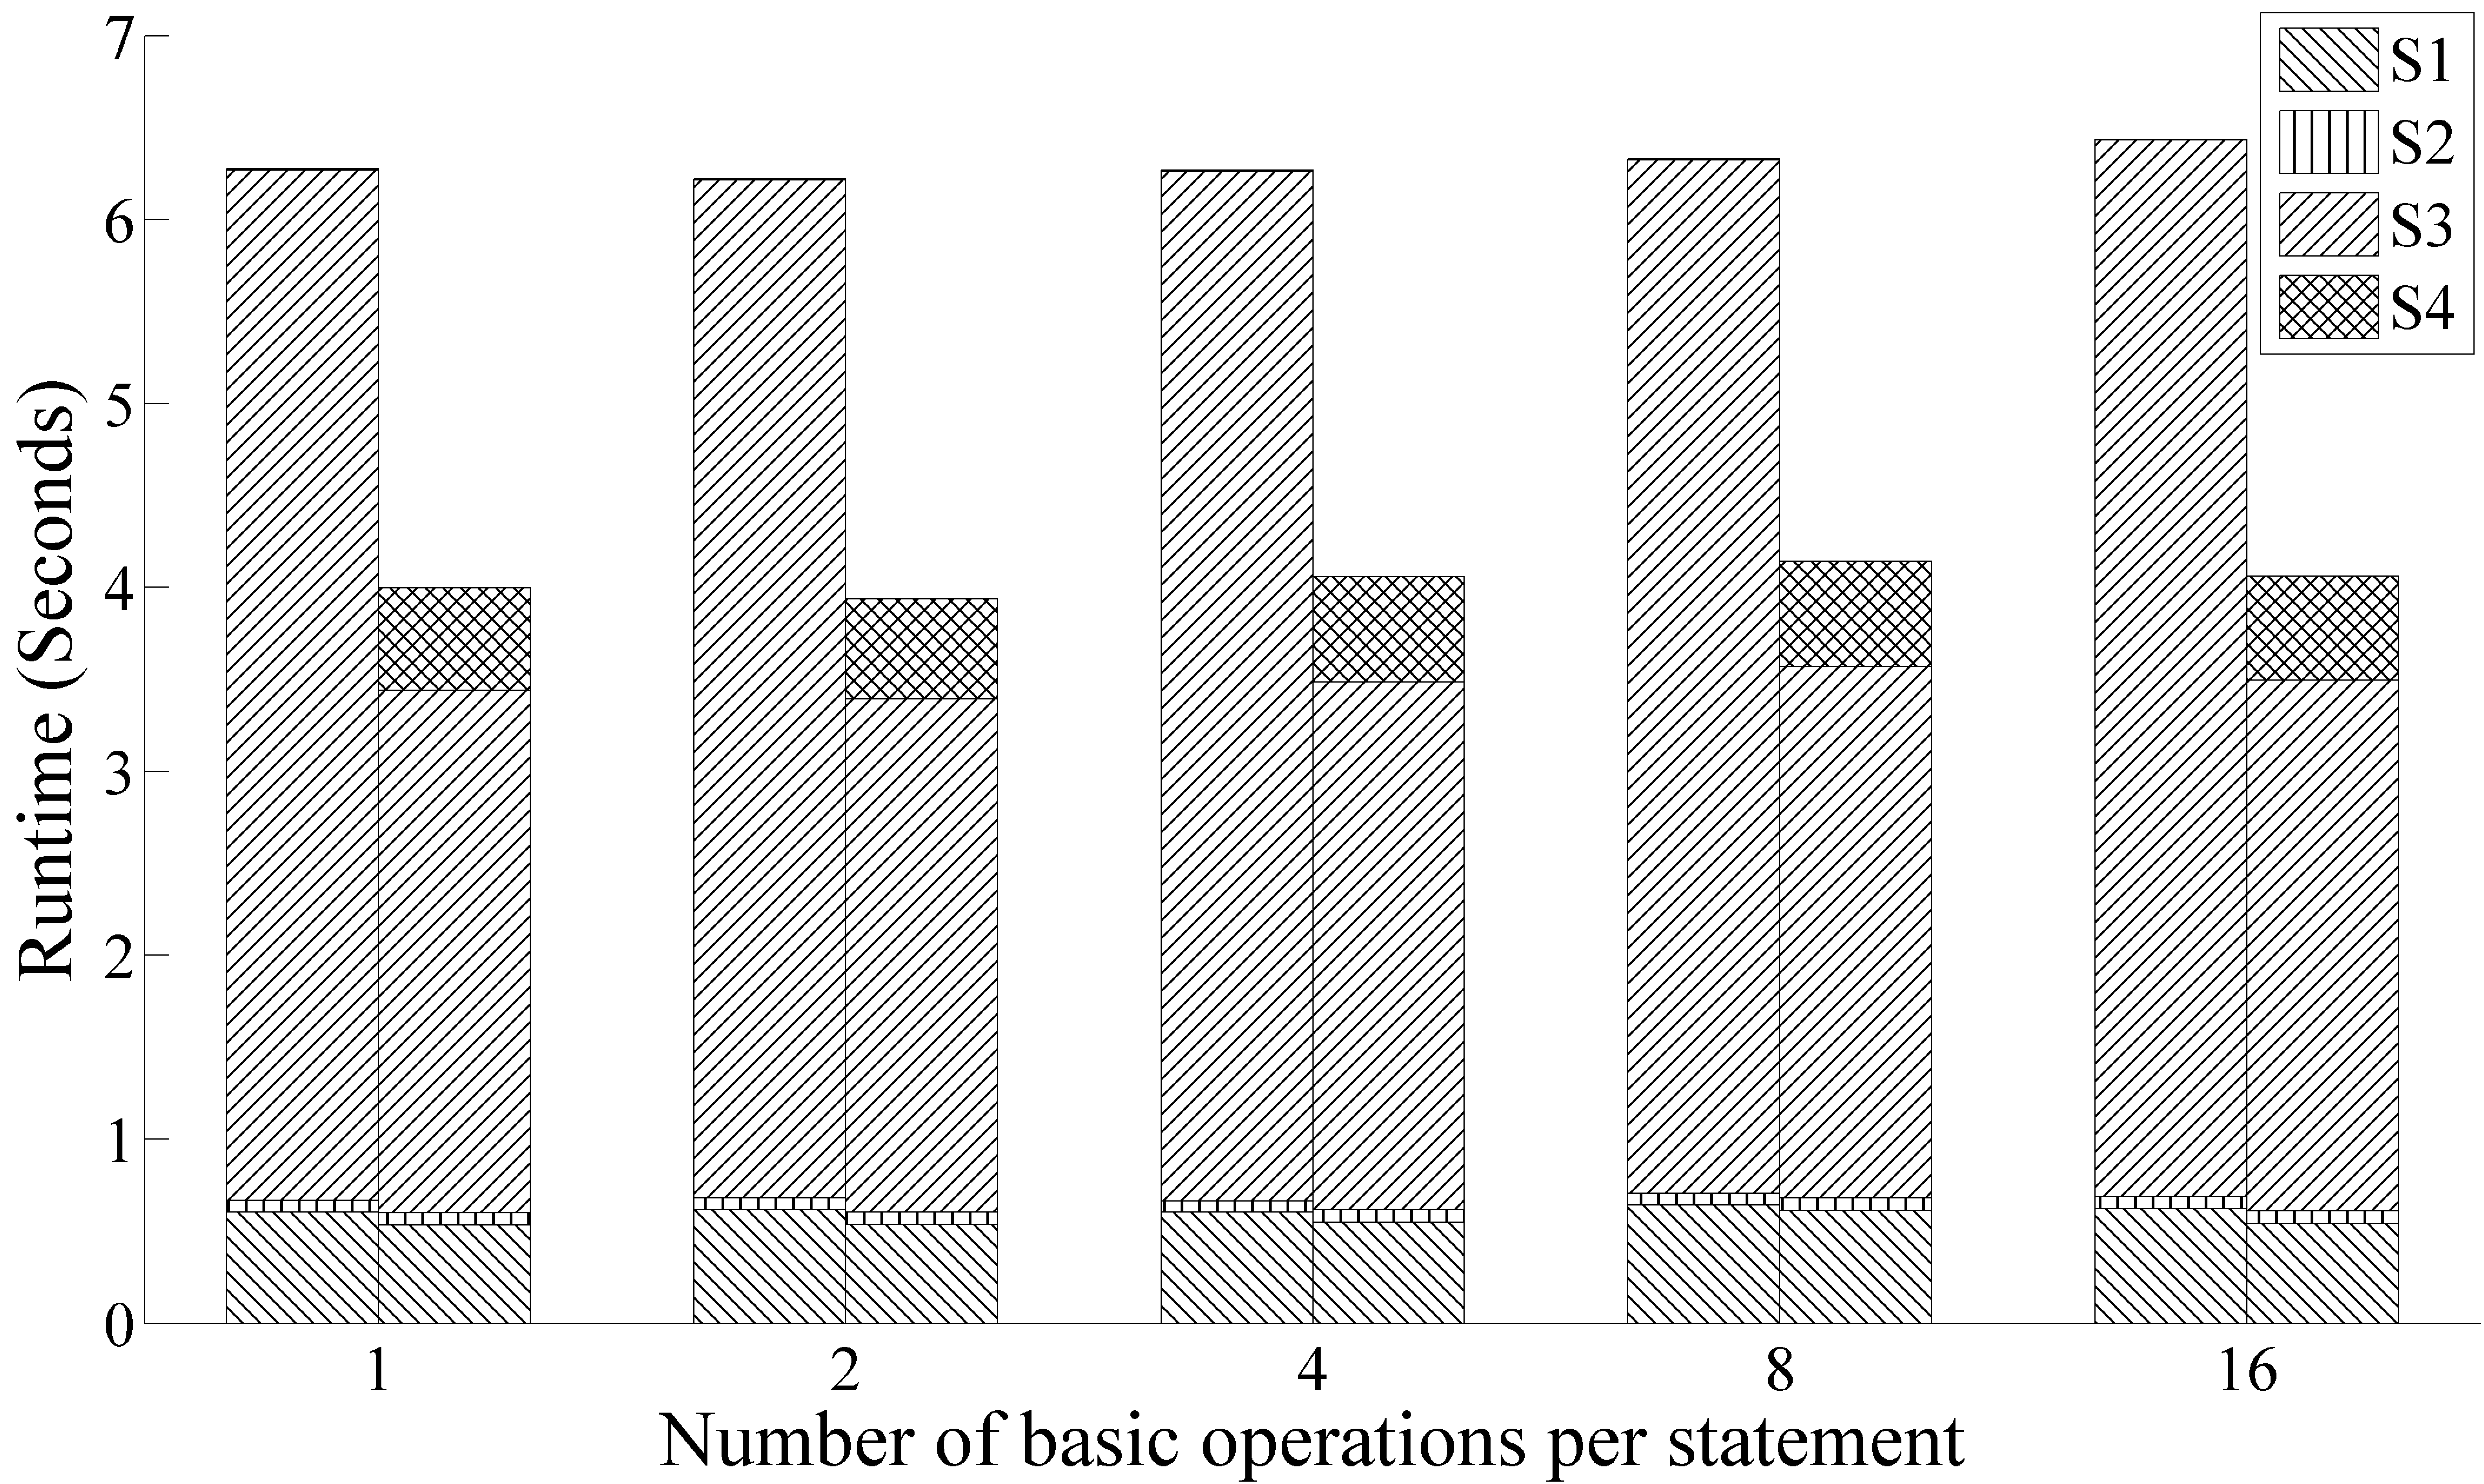
\includegraphics[width=1\textwidth]{figures/HRfig2BW}
\caption[Performance Breakdown for {\tt Direct} and {\tt Indirect} under Varying Number of Basic Operations per Loop]
{Performance breakdown for {\tt Direct} (left bar) and {\tt Indirect} methods. 
Fixed parameters: $n=20,000$, $\overline{\rho} = 6$, $B=16$. }
\label{fig:random-fig2}
\end{minipage}
\end{figure}


Figure~\ref{fig:random-fig1} shows runtime plots for the algorithms {\textsc{Livarh} and \textsc{Livarhacc} as well as
{\tt Direct} and {\tt Indirect} under this setting. We can see that {\tt Direct}, {\tt Indirect} and \textsc{Livarh} are insensitive to how the function is implemented, whereas \textsc{Livarhacc} is sensitive. In particular, the runtime of \textsc{Livarhacc} first goes down as the number of basic operations per statement increases, and then goes up. This happens because as we put 
more and more operations in a statement, we are creating more local updates and reducing the global updates.
Meanwhile the cost of each local update also increases.
As a result, \textsc{Livarhacc} performs the best when the number of operations per statement $k$ has some intermediate value, in this case, around $8$.
Beyond $k=8$, the runtime keeps increasing, and when $k=128$, \textsc{Livarhacc} surpasses \textsc{Livarh} in total runtime.


As already noted, changing $k$ does not affect the total runtime for the methods
{\tt Direct} and {\tt Indirect}. It would be interesting to see if it affects the runtime of 
any of the four constituent steps in these methods. 
In Figure~\ref{fig:random-fig2} we show the runtime breakdown for the four steps in these methods. The depicted results are for the same setting as in the previous test except that, in order to simplify the problem, we fix the total number of basic operations per loop ($B$) as $16$. We can see that changing $k$, the number of operators per statement, does not affect the runtime of any of the four steps in {\tt Direct} and {\tt Indirect}. These results are in accordance with expectation. For {\tt Direct}, the complexity of the coloring step $S2$ and the recovery step $S4$ depend only on the size and structure of the final Hessian matrix, and in general, these steps are negligible in terms of runtime compared to the steps $S1$ and $S3$. The compressed Hessian computation step $S3$ dominates the overall runtime. For {\tt Indirect}, $S2$ and $S4$ each take more time than their corresponding steps in {\tt Direct}. The step $S3$ in {\tt Indirect} takes much less time than the counterpart in {\tt Direct}, causing {\tt Indirect} to be faster than {\tt Direct}. The reason is because the time needed in $S3$ is proportional to the number of colors needed,
which in this particular case is $13$ for star coloring ({\tt Direct}) and 
$7$ for acyclic coloring ({\tt Indirect}). 

\paragraph{C) Scalability with respect to function complexity.}

We also studied the performance of these methods as we increase the complexity of the function. Since we have seen that \textsc{Livarhacc} performs the best when $k=8$, we fix $k$ to be $8$, and vary the number of statements per loop---in particular, we double the number each time. 
We use the runtime when there is only one statement per loop as a normalizing factor. 
Figure~\ref{fig:random-fig3} shows the results. 
\begin{figure}[htbp]
        \centering
        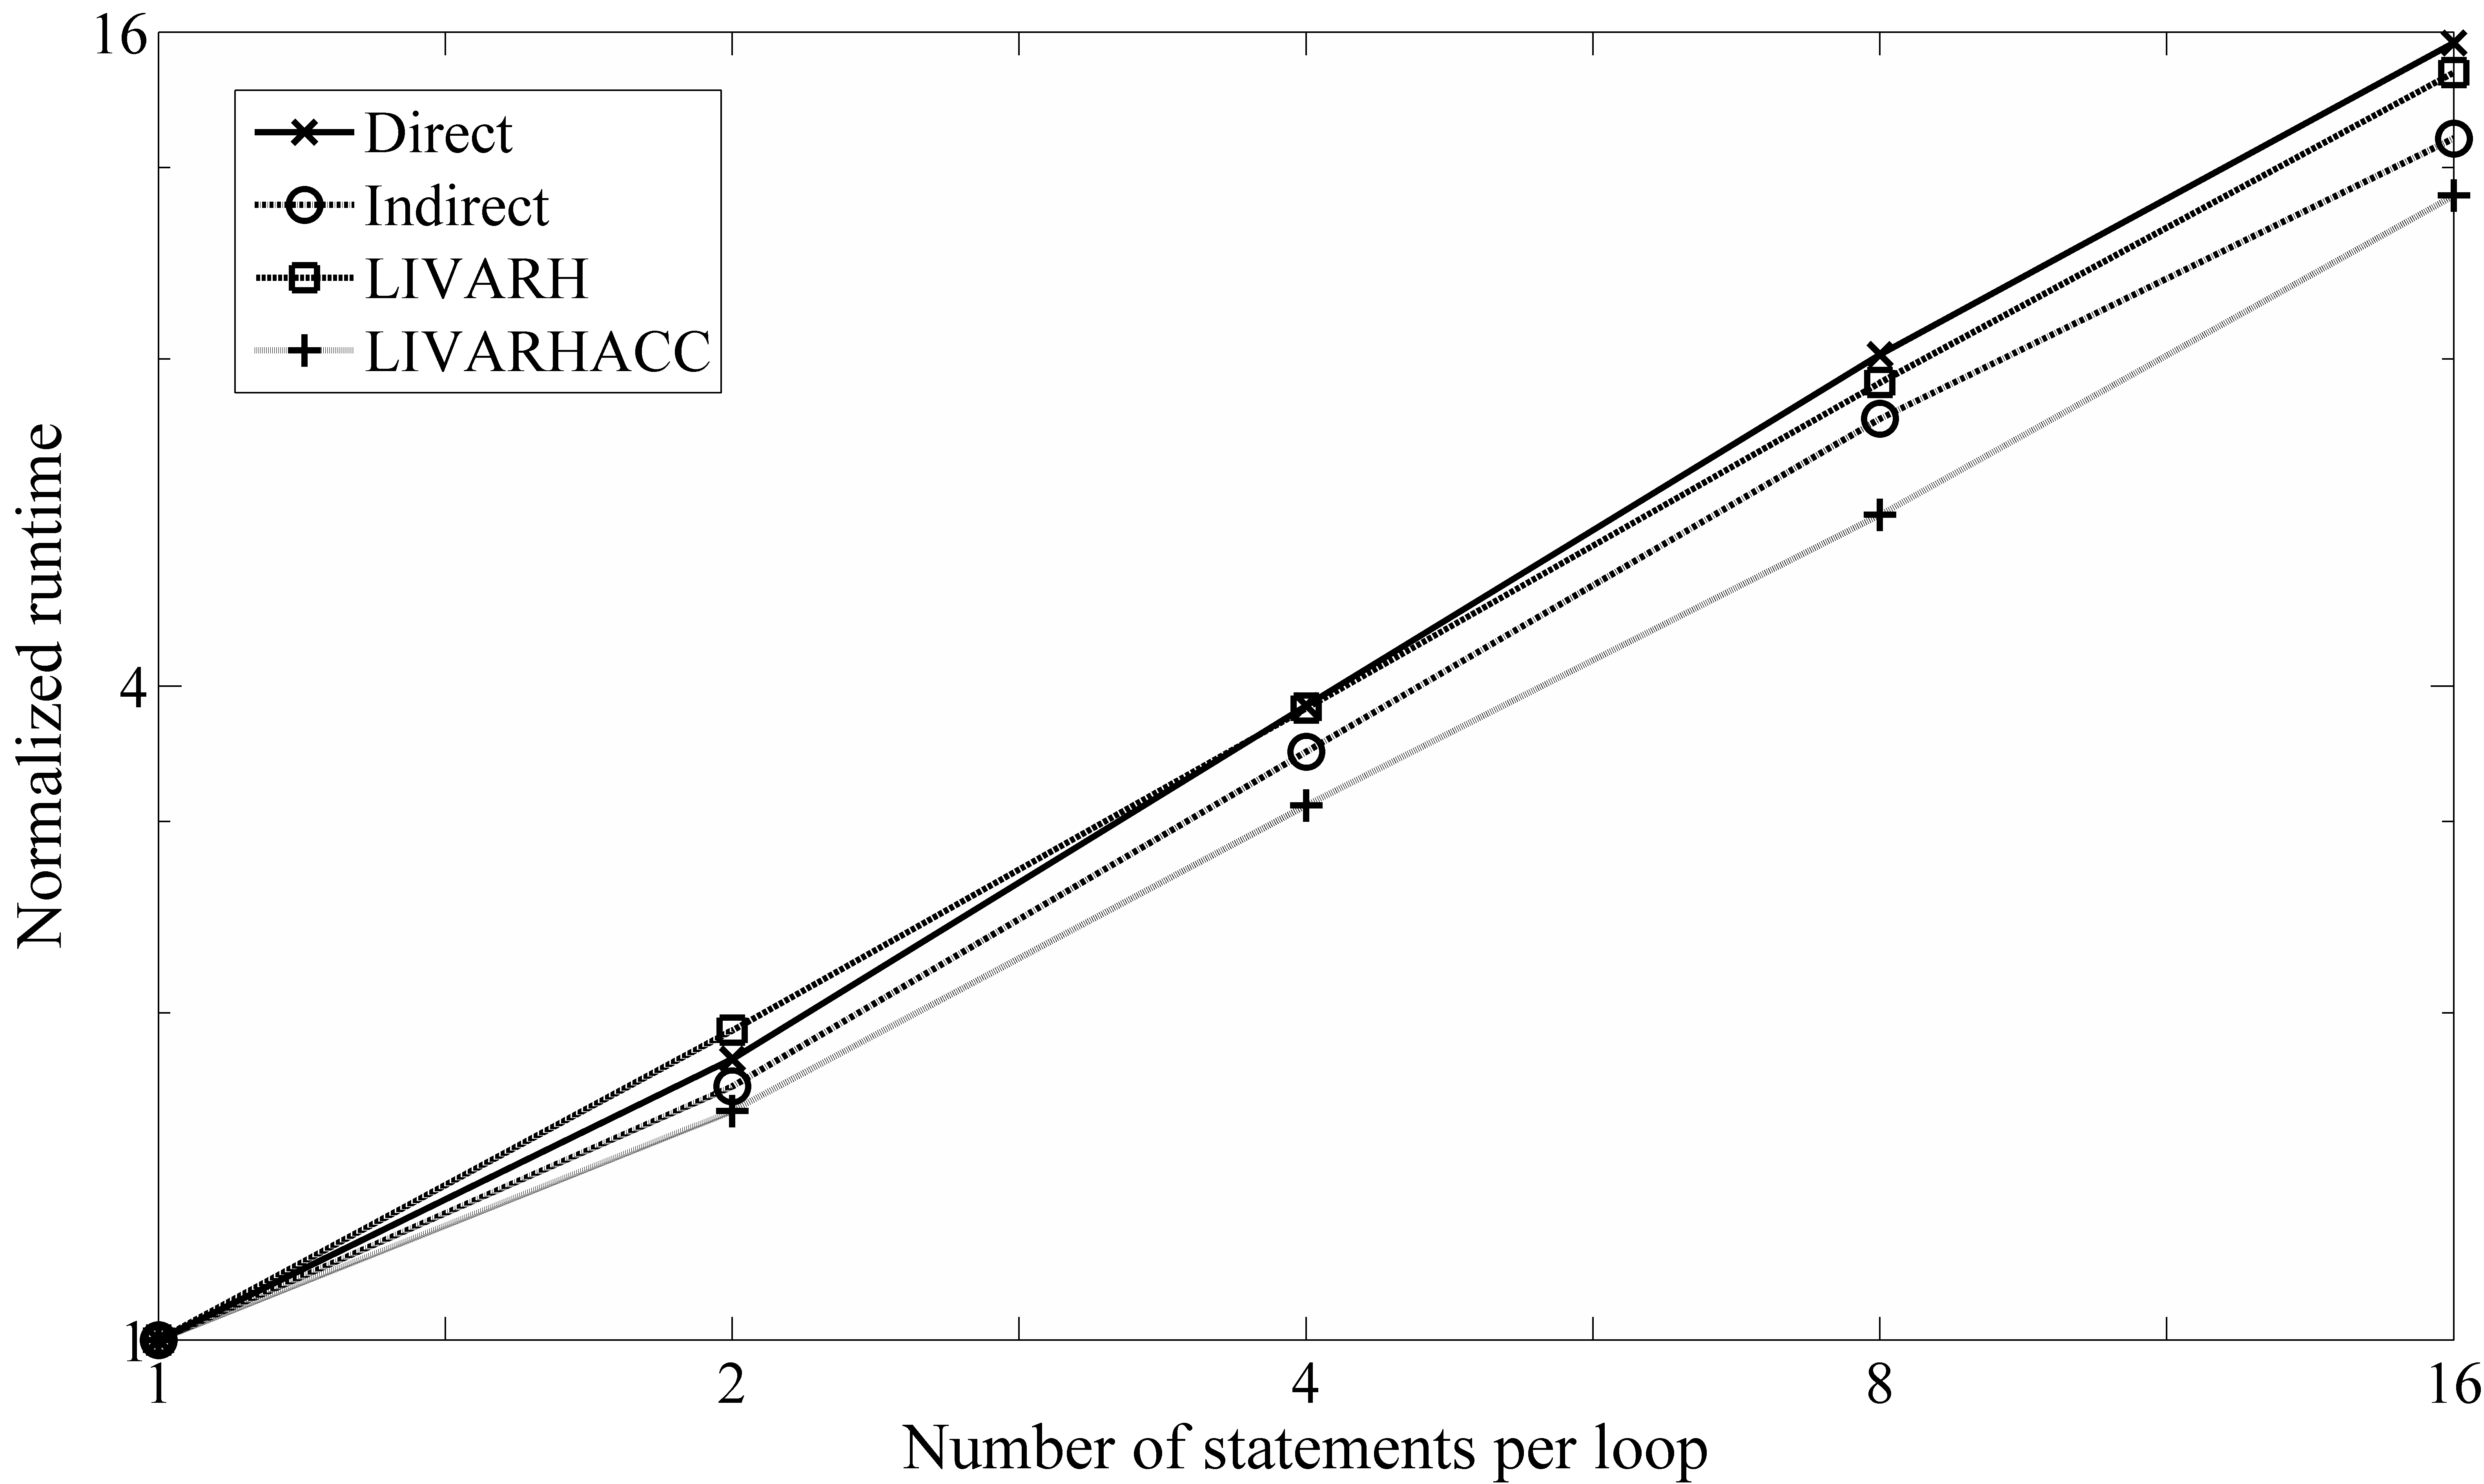
\includegraphics[width=0.65\textwidth]{figures/HRfig3BW}
        \caption[Scalability of the Different Algorithms Relative to Function Complexity]
                     {Scalability of the different algorithms relative to function complexity.}
        \label{fig:random-fig3}
\end{figure}

We observe, first, that all of these methods show linear scalability. More specifically, none of the methods needed more than twice the runtime when the complexity of the function evaluation is doubled. Further, we see that {\tt Indirect} and \textsc{Livarhacc} exhibit slightly super-linear scalability, that is, they require less than twice the runtime when doubling the complexity of the function evaluation. For {\tt Indirect}, this is because the runtime of neither the coloring step $S2$ nor the recovery step $S4$  changes when the number of statements per loop is doubled. For \textsc{Livarhacc}, the reason is when the number of identical statements in a loop increases, locality of memory accesses also increases. 


\paragraph{D) Dependence on sparsity of the final Hessian.}

In our last test, we tested how the sparsity of the final Hessian affects performance. Here, we vary the number of rows in the Hessian and approximately fix the total number of nonzeros by assigning different number of nonzeros per row in each case. We also fix the number of basic operators per loop as $8$ and the number of statements per loop as $2$. Table~\ref{tab:random-sparse} gives the structural properties of the resulting Hessian matrices.

\begin{table}[htbp]
\begin{center}
\caption[Structural Properties of Random Hessians with Varying Density but Constant $nnz$ ]
{Structural properties of random Hessians with varying density but fixed number of nonzeros.}
\label{tab:random-sparse}
\begin{tabular}{ | c | c | c | c | c | c |}
\hline
$n$ & avg & $\max$ &  $\min$ & No. colors & No. colors \\
&  $\lceil nnz/row \rceil$ &  $\lceil nnz/row \rceil$ &  $\lceil nnz/row \rceil$ & (star) & (acyclic) \\
\hline
10,000 & 12 & 25 & 6 & 26 & 11 \\
15,000 & 8 & 17 & 4 & 17 & 8 \\
20,000 & 6 & 15 & 3 & 13 & 7 \\
30,000 & 4 & 12 & 2 & 11 & 5 \\
\hline
\end{tabular}
\end{center}
\end{table}



\begin{figure}[htbp]
\centering
\begin{minipage}[b]{0.48\linewidth}
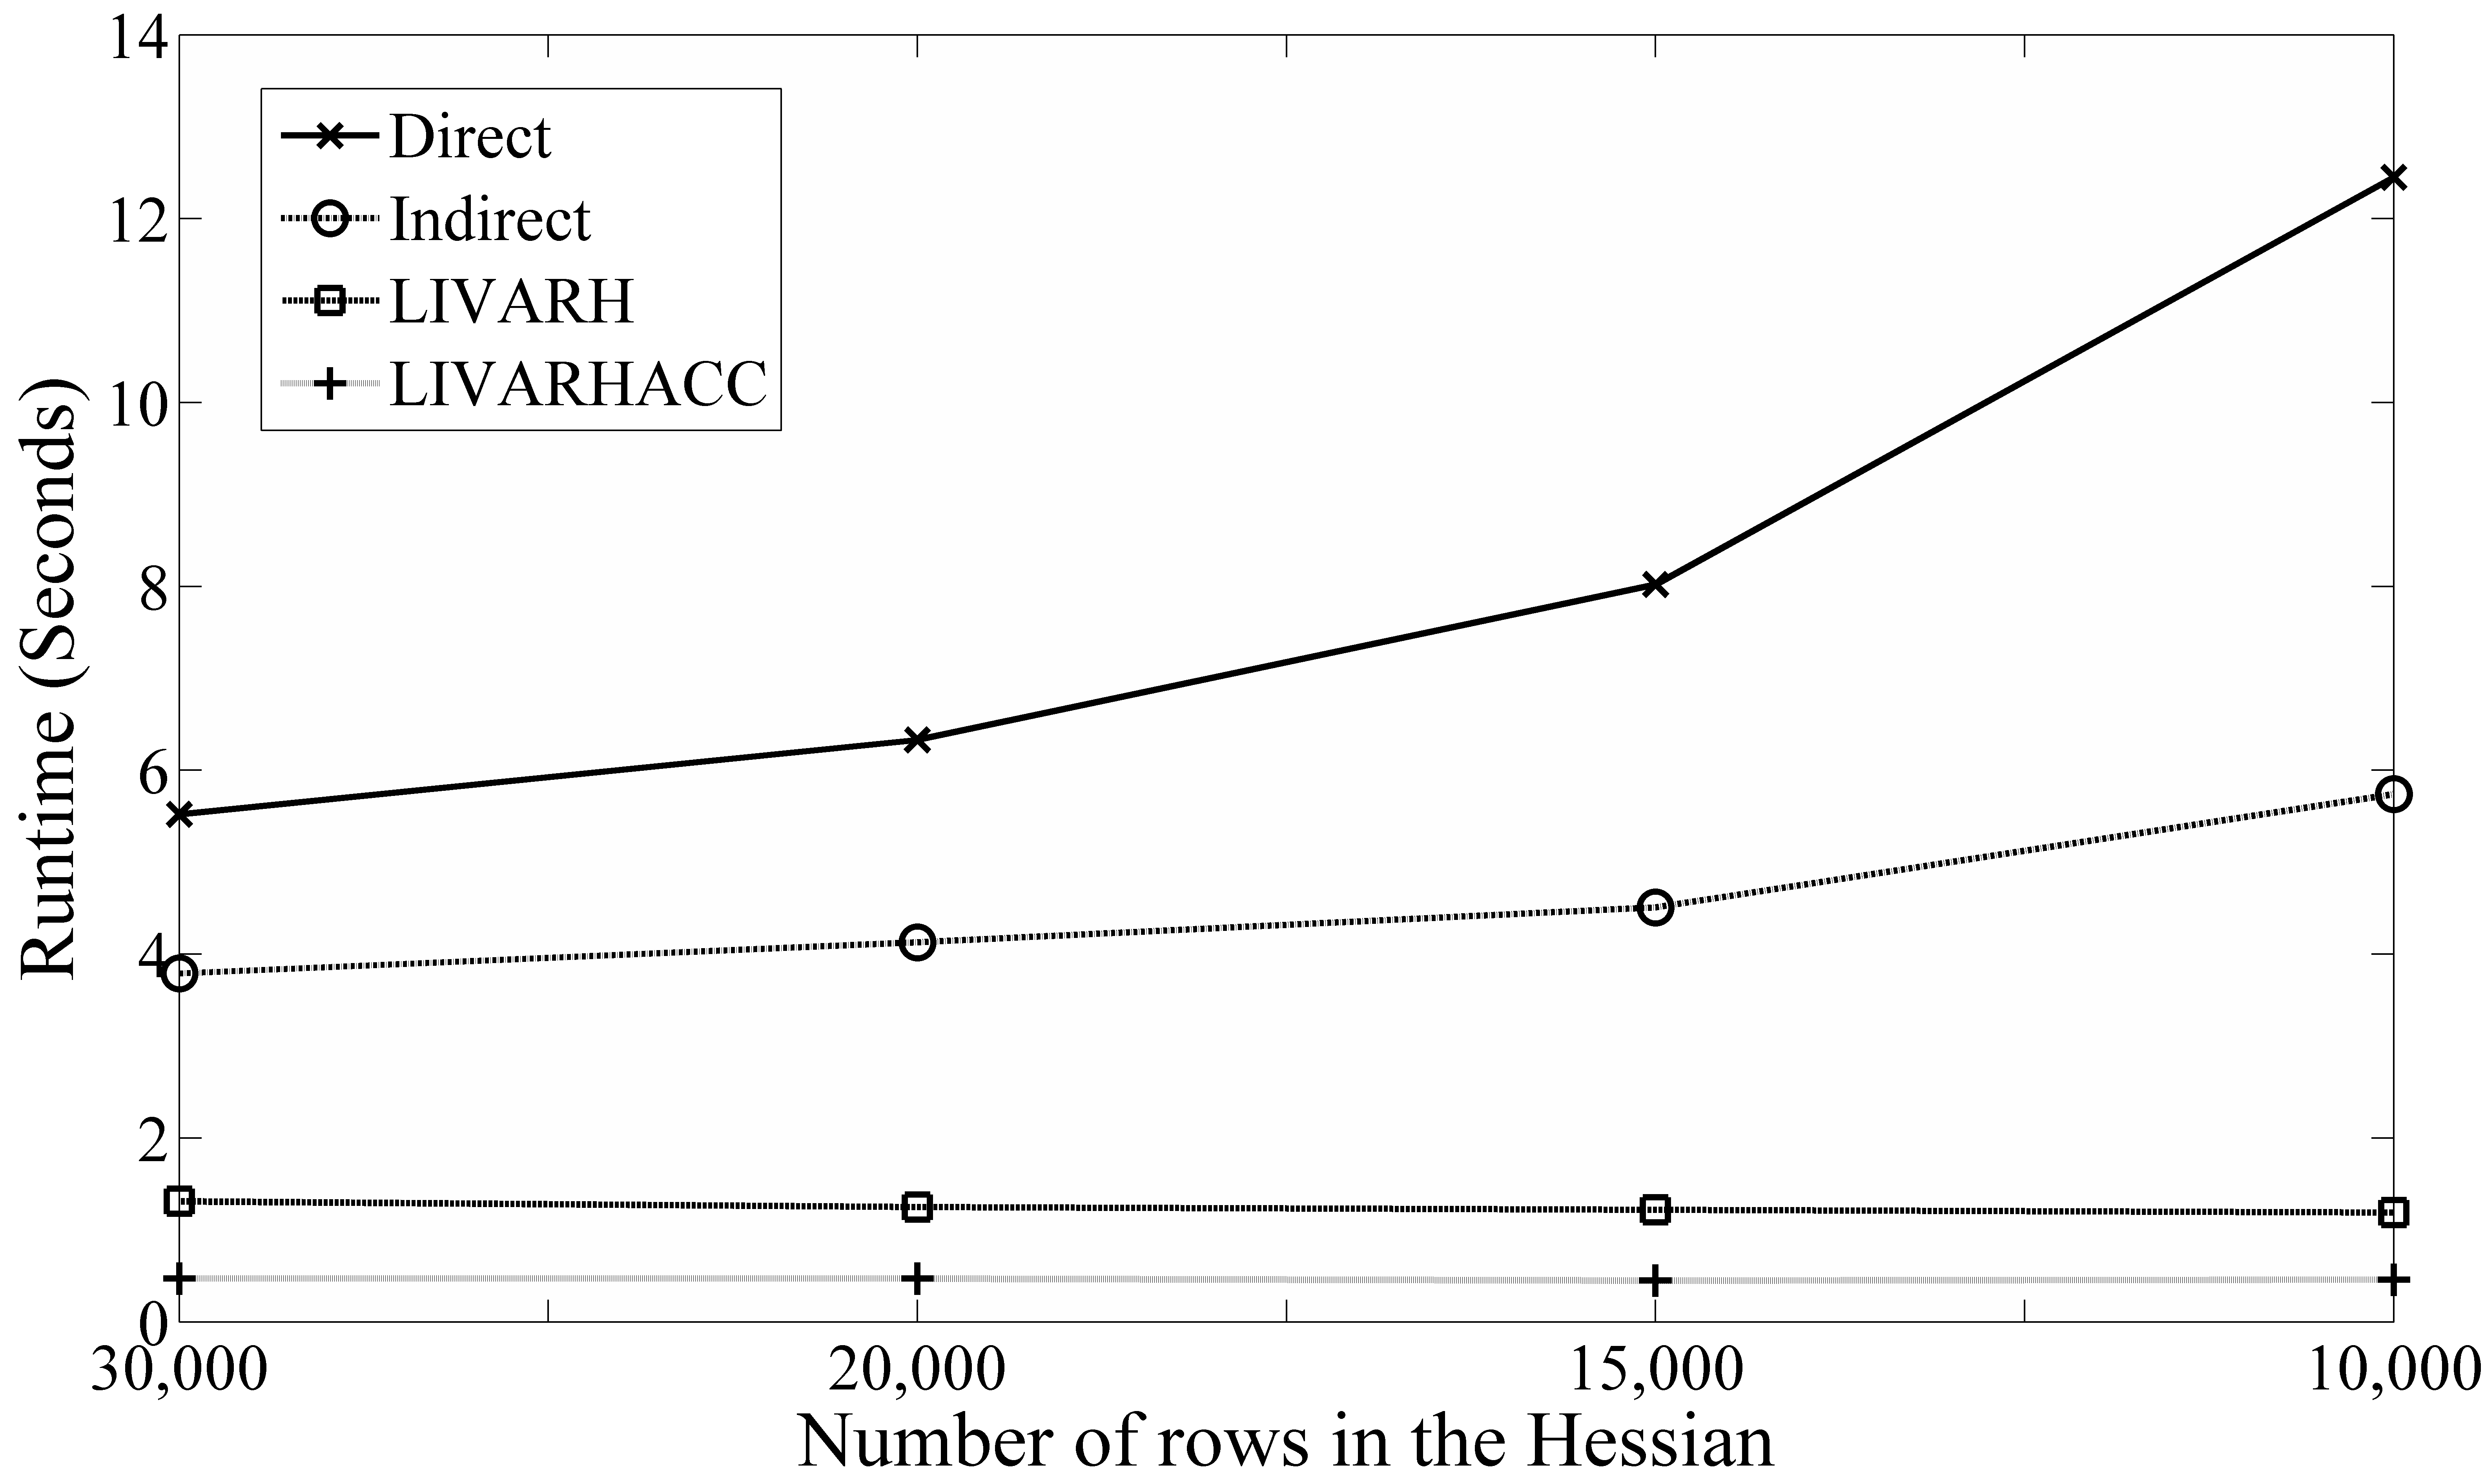
\includegraphics[width=1\textwidth]{figures/HRfig4BW}
\caption[Runtime Variation Under Different Density of Hessians]
{Runtime variation under different density of Hessians (fixed total number of nonzeros). See Table~\ref{tab:random-sparse} for structural data.}
\label{fig:random-fig4}
\end{minipage}
\quad
\begin{minipage}[b]{0.48\linewidth}
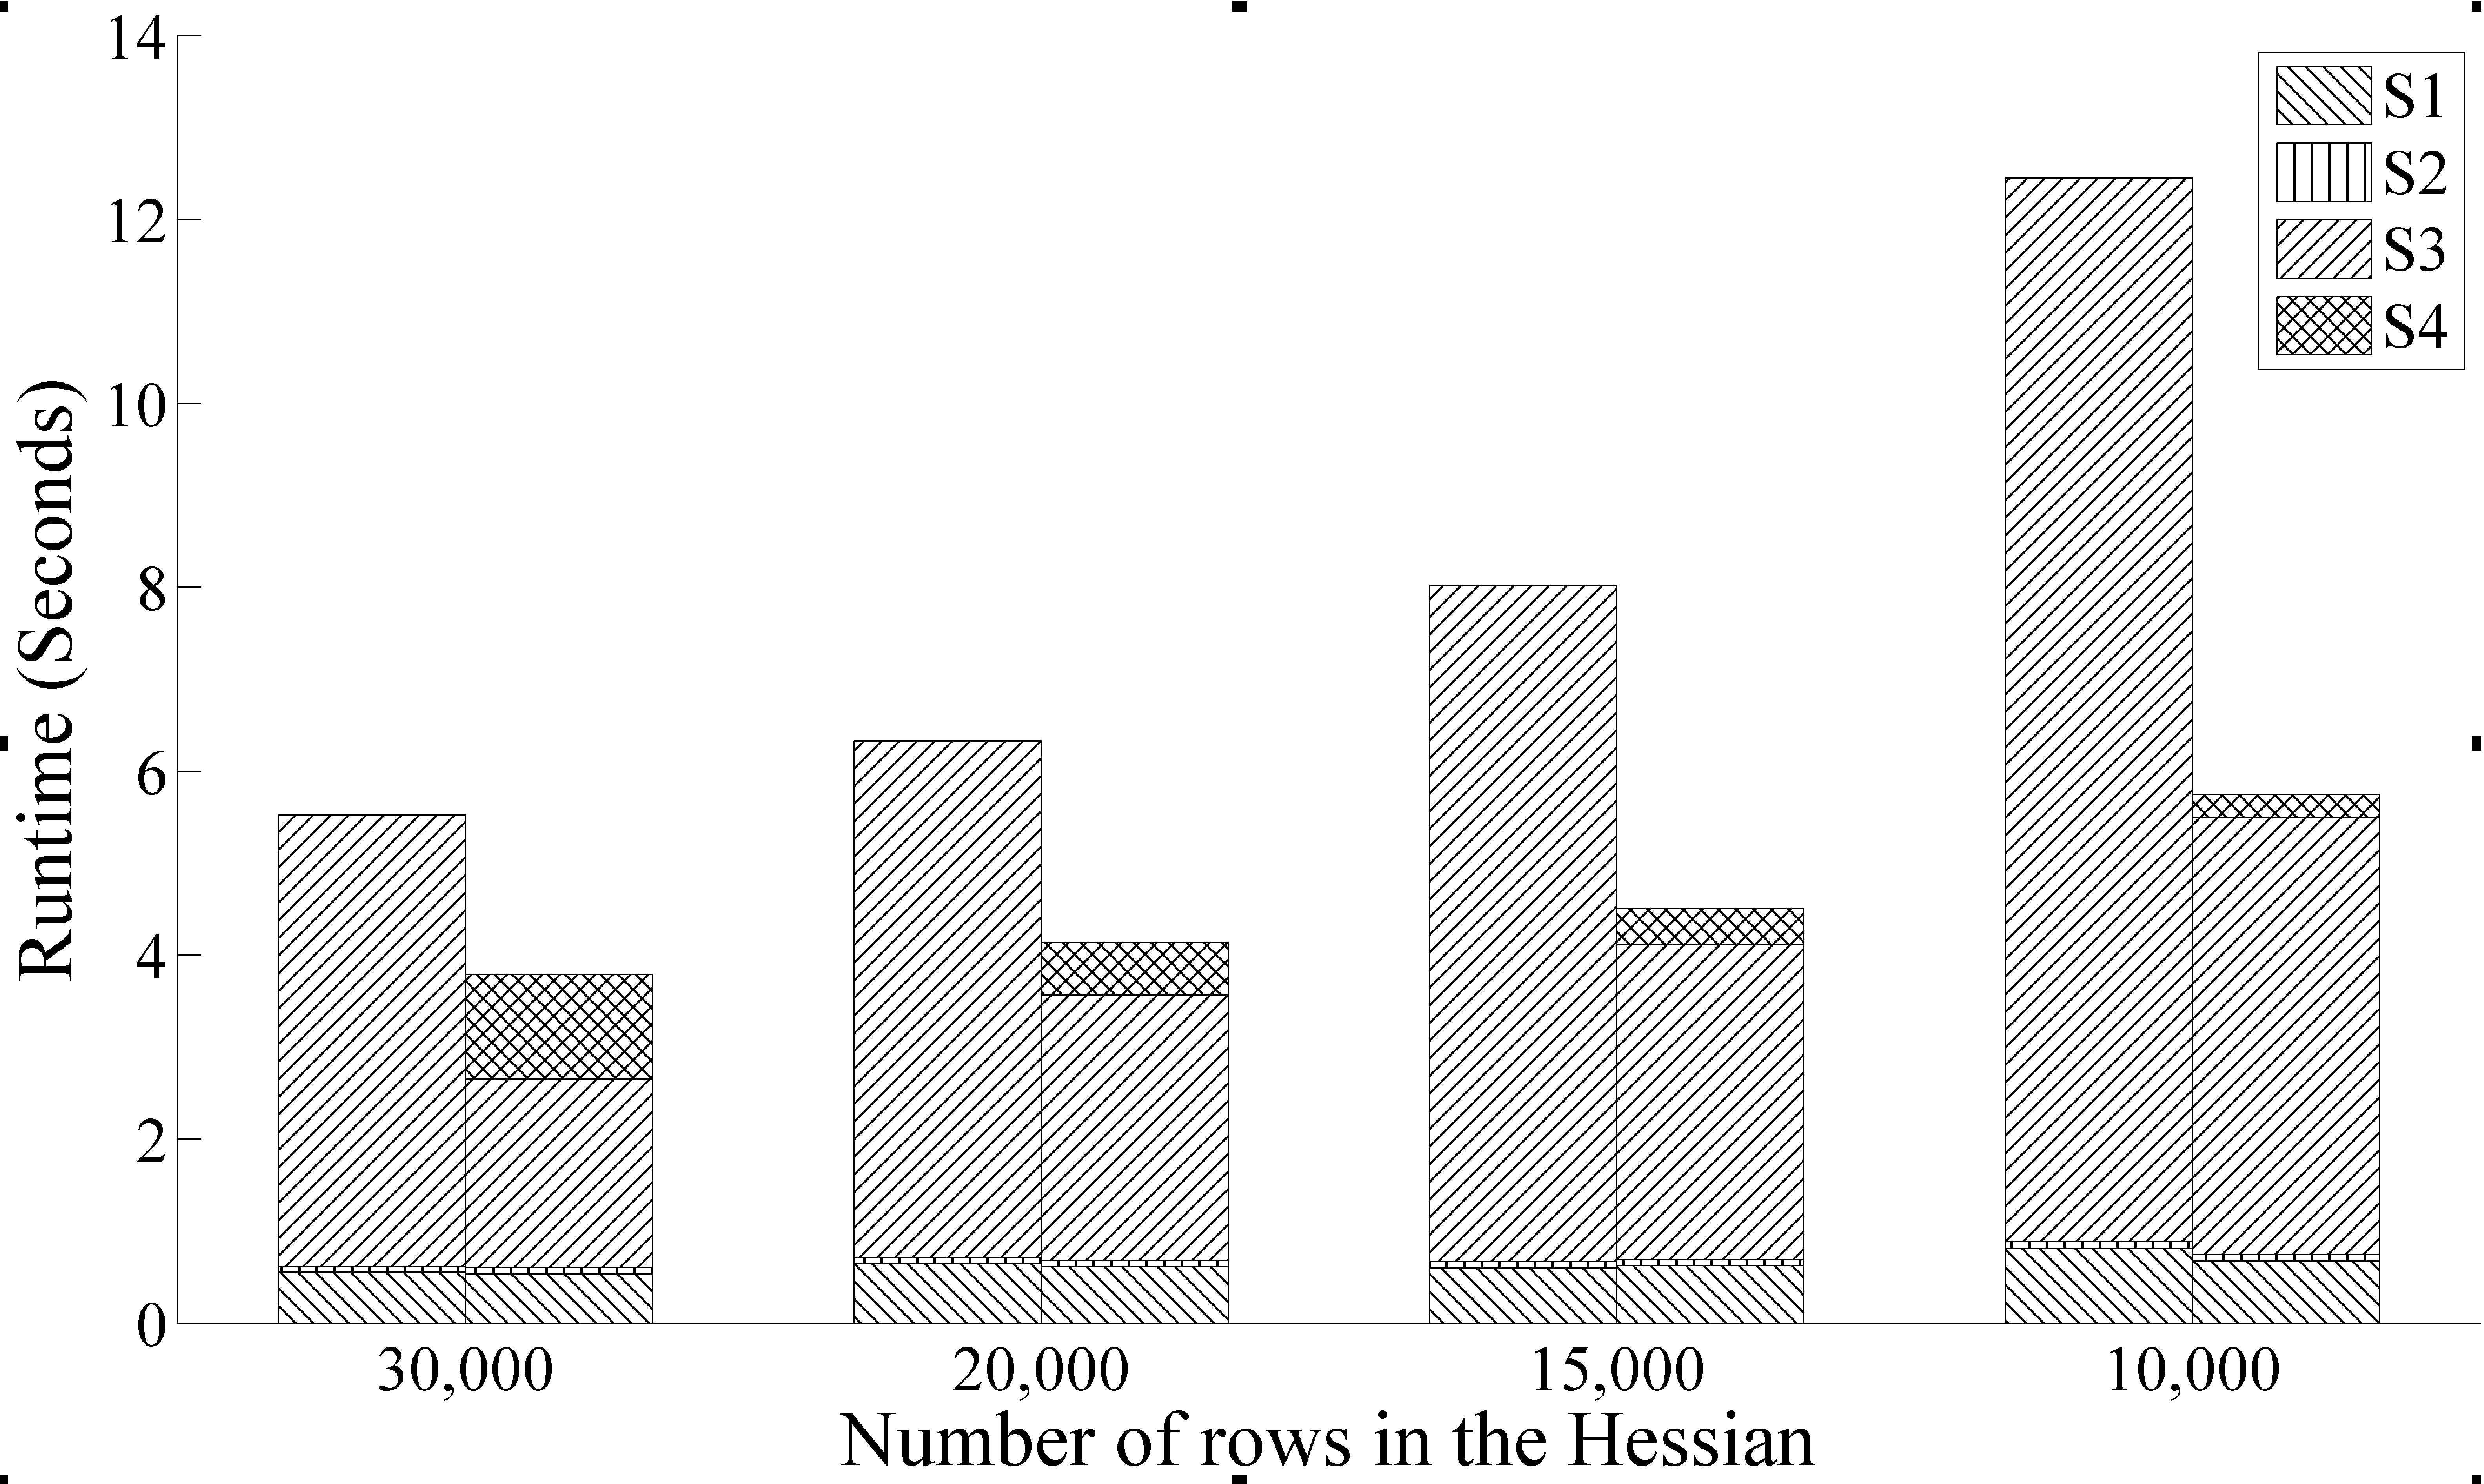
\includegraphics[width=1\textwidth]{figures/HRfig5BW}
\caption[Performance Breakdown for {\tt Direct} and {\tt Indirect} under 
Varying Density of Hessians]
{Performance breakdown for {\tt Direct} (left bar) and {\tt Indirect} (right bar) methods. Same data as in Figure~\ref{fig:random-fig4}.}
\label{fig:random-fig5}
\end{minipage}
\end{figure}

Figure~\ref{fig:random-fig4} shows runtimes for \textsc{Livarh}, \textsc{Livarhacc},
{\tt Direct} and {\tt Indirect} under this setting. 
It can be seen that the performances of \textsc{Livarh} and \textsc{Livarhacc} 
are unaffected by the changes in density. This is as expected because the complexity of these
algorithms is only determined by the number of SACs. The runtime of {\tt Direct} and {\tt Indirect} increases as the density of the Hessian matrix increases. Figure~\ref{fig:random-fig5} shows the runtime breakdown for {\tt Direct} and {\tt Indirect}. For {\tt Direct} the runtime 
is dominated by step $S3$, which in turn is proportional to the number of colors needed. As the Hessian size is decreased while keeping the total number of nonzeros fixed, the matrix gets denser and so we need more colors. As a result, {\tt Direct} would need more time to evaluate the compressed Hessian. For {\tt Indirect}, the runtime for the recovery step $S4$ decreases when we have a Hessian matrix of smaller size, but the increase in the time for step $S3$ still dominates the overall runtime.


\bibliographystyle{abbrv}
\bibliography{adbib}

\end{document}